\PassOptionsToPackage{unicode,pdfusetitle}{hyperref}
\PassOptionsToPackage{hyphens}{url}
\PassOptionsToPackage{dvipsnames}{xcolor}

\documentclass[english,a4paper]{article}

\usepackage{geometry}

% Font settings
\usepackage[T1]{fontenc}
\usepackage{lmodern}
\usepackage{amssymb,amsmath,amsthm,mathtools}
\usepackage{textcomp}
\usepackage{csquotes}
\usepackage{babel}
\usepackage{upquote}

\usepackage[textsize=footnotesize]{todonotes}

\usepackage{microtype}
\UseMicrotypeSet[protrusion]{basicmath} % disable protrusion for tt fonts

% Colors
\usepackage{xcolor}

% Hyperlinks, urls, etc
\usepackage{xurl}

\usepackage{hyperref}
\hypersetup{
  colorlinks = true,
  breaklinks = true,
  linkcolor  = black,
  filecolor  = MidnightBlue,
  citecolor  = MidnightBlue,
  urlcolor   = MidnightBlue
}

\usepackage{cleveref}

% Floats
\usepackage{graphicx}
\usepackage{booktabs}
\usepackage{caption}
\usepackage{subcaption}

% Algorithms
\usepackage{algorithm,algpseudocode}

% Title Page
\usepackage[]{authblk}
\renewcommand\Affilfont{\itshape\small}

\setlength{\emergencystretch}{3em} % prevent overfull lines

% operators
\DeclareMathOperator*{\argmax}{arg\,max}
\DeclareMathOperator*{\argmin}{arg\,min}
\DeclareMathOperator{\E}{E}
\DeclareMathOperator{\var}{Var}
\DeclareMathOperator{\cov}{Cov}
\DeclareMathOperator{\tr}{tr}
\DeclareMathOperator{\diag}{diag}
\DeclareMathOperator{\range}{range}
\DeclareMathOperator{\nullspace}{null}
\DeclareMathOperator{\rank}{rank}
\DeclareMathOperator{\card}{card}
\DeclareMathOperator{\sign}{sign}
\DeclareMathOperator{\st}{S}
\DeclareMathOperator{\normal}{Normal}
\DeclareMathOperator{\fnormal}{FoldedNormal}
\DeclareMathOperator{\bernoulli}{Bernoulli}
\DeclareMathOperator{\erf}{erf}
\DeclareMathOperator{\mse}{MSE}
\DeclareMathOperator{\risk}{R}
% \DeclareMathOperator{\I}{I}
% \DeclareMathOperator{\T}{}
%
% \DeclareMathSymbol{\phi}{\mathalpha}{operators}{0}
\DeclareMathOperator{\pdf}{\phi}
\DeclareMathOperator{\cdf}{\Phi}
% commands
% \newcommand{\vec}{\vectorsym}
% \newcommand{\mat}{\matrixsym}
\renewcommand{\vec}{\boldsymbol}
\newcommand{\mat}{\boldsymbol}
\newcommand*\du{\mathop{}\!\mathrm{d}}
% \newcommand{\T}{\mathsf{T}}
\newcommand{\T}{\intercal}
\newcommand{\ones}{\boldsymbol{1}}
% \newcommand{\T}{\intercal}
% \newcommand{\T}[1]{{1}^{\mathsf{T}}}
\newcommand{\ind}[1]{\operatorname{I}_{#1}}

% environments
\theoremstyle{plain}
\newtheorem{theorem}{Theorem}[section]
\newtheorem{corollary}{Corollary}[theorem]
\newtheorem{lemma}{Lemma}[section]
\newtheorem{proposition}{Proposition}[section]

\theoremstyle{definition}
\newtheorem{definition}{Definition}[section]
\newtheorem{example}{Example}[section]

\theoremstyle{remark}
\newtheorem{remark}[theorem]{Remark}

\newcommand{\todojl}[1]{\todo[color=green!40]{#1}}



\newcommand{\mv}[1]{{\boldsymbol{\mathrm{#1}}}}

% title block
\title{Standardization and Regularization}
\author[1,*]{Johan Larsson}
\affil[1]{Department of Statistics, Lund University}
\affil[*]{Corresponding author:
  \href{mailto:johan.larsson@stat.lu.se}{\nolinkurl{johan.larsson@stat.lu.se}}
}
\date{\today}

% bibliography
\usepackage[style=alphabetic]{biblatex}
\addbibresource{normreg.bib}

\begin{document}

\maketitle

\section{Introduction}

When modeling high-dimensional high-dimensional where the number of features \(p\) exceeds
the number of observations \(n\), it is impossible to apply classical statistical models
such as standard linear regression since the design matrix \(\mat X\) is no longer of full
rank. A common remedy to this problem is to \emph{regularize} the model by adding a term to
the objective function that punishes models with large coefficients (\(\vec\beta\)). If we
let \(g(\vec\beta; \mat X, \vec y)\) be the original objective function---which when
minimized improves the model's fit to the data (\(\mat X, \vec y\))---then we are
interested in minimizing the following objective:
\begin{equation}
  \label{eq:general-objective}
  f(\beta_0, \vec\beta; \mat X, \vec y) = g(\beta_0, \vec\beta; \mat X, \vec y) + h(\vec\beta),
\end{equation}
which is composed of \(g\) and a penalty term \(h(\vec\beta)\) that depends only on \(\bm{\beta}\).
Some of the most common penalties are the \(\ell_1\) norm (\(\lVert \vec\beta \rVert_1\)) and squared \(\ell_2\) norm
penalties (\(\lVert \bm{\beta} \rVert_2^2\)), which if \(g\) is the standard ordinary least-squares objective, represent
the lasso~\citep{tibshirani1996,santosa1986,donoho1994} and ridge (Tikhonov) regression
% TODO: insert reference for ridge regression
respectively. Other common penalties include the sorted \(\ell_1\)-norm used in Sorted
L-One Penalized Estimation (SLOPE)~\citep{bogdan2013,zeng2014,bogdan2015}, the
minimax-concave penalty (MCP)~\citep{zhang2010}, hinge loss (used in support vector
machines~\citep{cortes1995}) and smoothly-clipped absolute
deviation~(SCAD)~\citep{fan2001}. Many penalities---indeed all of the mentioned
ones---shrink coefficients in proportion to their sizes.

The issue with this type of shrinkage is that it is sensitive to the scales of the features
in \(\mat X\). To avoid this it is common to \emph{normalize} the features before fitting
the model by shifting and scaling each feature by measures of location and scale
respectively. For some problems such measures arise naturally from contextual knowledge
about the problem, but in most cases they must be estimated from data. A popular strategy
is to use the mean and standard deviation of each feature as location and scale factors
respectively, which is called \emph{standardization}. Most types of normalization are based
only on the marginal distributions of the features, but there are exceptions such as the
adaptive lasso~\citep{zou2006}. Another reason for normalizing the features is to improve
properties of optimization algorithms used to fit the model, but we will not consider this
topic here.

The choice of normalization may have consequences for the estimated model. As a first
example of this, consider \Cref{fig:realdata-paths}, which displays the lasso paths for
four real data sets and two different types of normalization. For most of the datasets, the
models differ significantly depending on type of normalization, yielding differences in
terms of feature selection as well as signs and magnitudes of the corresponding
coefficients.

% TODO: reduce image to one row?
\begin{figure}[bpt]
  \centering
  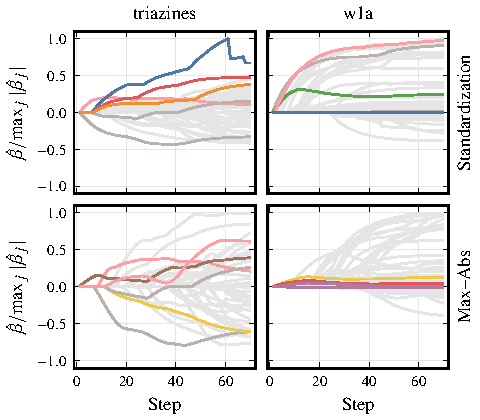
\includegraphics[]{plots/realdata_paths_small.pdf}
  \caption{%
    Lasso paths for real datasets using two types of normalization:
    standardization and maximum absolute value normalization (max--abs). We have fit
    the lasso path to two different datasets:
    \data{triazines}~\citep{king} and \data{w1a}~\citep{platt1998}. (See \Cref{sec:data-summary}
    for more information about these data sets.) For each
    dataset, we have colored the coefficients if they were among the first five
    to become non-zero under either of the two normalization schemes.
  }
  \label{fig:realdata-paths}
\end{figure}

In spite of this relationship between normalization and regularization, there has so far
been no research on the topic. Instead, the choice of normalization is often motivated by
being standard. And sometimes the choice is based on computational aspects such as
optimization performance and data storage. At the time of writing, for instance, the
popular machine learning library \texttt{scikit-learn}~\citep{scikit-learndevelopers2024}
recommends maximum absolute value normalization in the particular case of sparse data. Yet,
as we have already seen (\Cref{fig:realdata-paths}), this may have dramatic effects for the
results.

Standardization is a natural choice when the features are normally distributed. But for
other types of data the choice is not as straightforward. There is for instance no clear
approach to normalizing binary features (where the each observations takes either of only
two values). Anecdotal suggestions include not normalizing at all or to normalize as you
would if it were continuous data---the implications of either of these suggestions (or in
deed any other), however, have yet to be investigated.

In this paper we will begin to bridge this knowledge gap by studying normalization in the
context of binary data. We will focus on three models that each correspond to a particular
case of \Cref{eq:general-objective}: the lasso, ridge, and elastic net~\citep{zou2005}. The
latter of these, the elastic net, is a generalization of the previous two, and is
represented by the following optimization problem:
%
\begin{multline}
  \label{eq:elastic-net}
  \operatorname*{minimize}_{\beta_0 \in \mathbb{R},\vec{\beta} \in \mathbb{R}^p}\bigg( f(\beta_0, \vec{\beta};\vec{X},\vec{y},\lambda_1,\lambda_2)= \\
  \frac{1}{2} \lVert \vec y - \beta_0 - \tilde{\mat{X}}\vec{\beta} \rVert^2_2  + \lambda_1 \lVert \vec\beta \rVert_1 + \frac{\lambda_2}{2}\lVert \vec \beta \rVert_2^2\bigg).
\end{multline}
%
Setting \(\lambda_1 = 0\) results in the ridge regression objective, whereas \(\lambda_2 =
0\) gives us the lasso. These methods are staples in the field of statistics and machine
learning and are accompanied by a large body of theoretical work and applications for real
data.

We pay particular attention to the case when binary features are imbalanced, that is, have
relatively many ones or zeroes. In this scenario, we demonstrate that the choice of
normalization directly influences the estimated regression coefficients and that this
effect is different for the lasso and ridge regression. In the case of the lasso, we show
that this bias can be mitigated by scaling with variance but that this comes at the cost of
increased variance. For ridge regression we show that scaling by standard deviation
achieves the same effect. In the case of the elastic net, however, we show that there is no
simple normalization method that can mitigate this bias but that it is possible to
circumvent it by instead weighting the penalty terms in the elastic net.

We also study the case of mixed data and show that the choice of normalization has implicit
consequences for the relative weighting of binary and normal features, even in the case
when the binary features are balanced. If we believe, for instance, that a unit change in
the binary variable should equal a certain change in the normal variable (say, two standard
deviations), then scaling must be modified to take this into account.

% TODO: complete this paragraph
Finally, we look at a simple case of interactions between normal and binary features, and
demonstrate what?


\section{Preliminaries}

Throughout this paper, we assume that the data is generated from a linear model, \(y_i =
\beta_0^* + \vec x_i^\T \vec\beta^* + \varepsilon_i\) for \(i \in [n]\) where \([n] =
\{1,2,\dots,n\}\) and we use \(\beta_0^*\) and \(\vec\beta^*\) to denote the true intercept
and coefficients, respectively, and \(\varepsilon_i\) to denote measurement noise. \(\mat
X\) is the \(n \times p\) design matrix with features \(\vec x_j\) and \(\vec y\) the \(n
\times 1\) response vector. Furthermore, we use \(\hat\beta_0\) and \(\hat{\vec{\beta}}\)
to denote our estimates of the intercept and coefficients. We will also assume \(\mat{X}\),
\(\beta_0^*\), and \(\vec{\beta}^*\) to be fixed.

There is considerable ambiguity regarding key terms in the literature. Here, we define
\emph{normalization} as the process of centering and scaling the feature matrix, which we
now formalize.

\begin{definition}[Normalization]
  \label{def:normalization}
  Let \(\tilde{\mat X}\) be the normalized feature matrix with elements
  \(\tilde{x}_{ij} = (x_{ij} - c_{j})/s_j\), where \(x_{ij}\) is an element of
  \(\mat{X}\) and \(c_j\) and \(s_j\) are the \emph{centering} and
  \emph{scaling} factors respectively.
\end{definition}

% Some authors refer to the procedure in \Cref{def:normalization} as \emph{standardization},
% but here we define standardization only as the case when centering with the mean and
% scaling with the (uncorrected) standard deviation.

\subsection{Types of Normalization}

There are many different strategies for normalizing the design matrix. We list a few common
choices in \Cref{tab:normalization-types}. Standardization is perhaps the most popular type
of normalization, at least in the field of statistics. One of its benefits is that it
simplifies certain aspects of fitting the model, such as fitting the intercept. The
downside of standardization is that it involves centering by the mean, which destroys
sparsity. This is not a problem when \(\bm{X}\) is stored as a dense matrix; but when the
data is sparse, it may increase memory use and processing time.

% TODO: move to appendix?
\begin{table}[hbt]
  \centering
  \caption{
    Common ways to normalize a matrix of features using centering and scaling
    factors \(c_j\) and \(s_j\), respectively. Note that \(\bar{x}_j =
    n^{-1}\sum_{i=1}^n x_{ij}\).
  }
  \label{tab:normalization-types}
  \vskip 0.15in
  \small
  \begin{tabular}{lll}
    \toprule
    Normalization            & \(c_{j}\)          & \(s_j\)                                                   \\
    \midrule
    Standardization          & \(\bar{x}_j\)      & \(\sqrt{\frac{1}{n}\sum_{i=1}^n (x_{ij} - \bar{x}_j)^2}\) \\
    \addlinespace
    Max--Abs                 & 0                  & \(\max_i|x_{ij}|\)                                        \\
    \addlinespace
    Min--Max                 & \(\min_i(x_{ij})\) & \(\max_i(x_{ij}) - \min_i(x_{ij})\)                       \\
    \addlinespace
    \(\ell_1\)-Normalization & 0 or \(\bar{x}_j\) & \(\lVert \vec{x}_j\rVert_1\)                              \\
    \addlinespace
    Adaptive Lasso           & 0                  & \(\hat{\beta}_j^\text{OLS}\)                              \\
    \bottomrule
  \end{tabular}
\end{table}

When the data is sparse, a common alternative to standardization is to scale features by
their maximum absolute values (max--abs normalization). This method has no impact on binary
data\footnote{Except in the extreme case when all values are 0.} and therefore retains
sparsity. For other types of data, it scales the features to take values in the range
\([-1, 1]\). Since the scaling is determined by a single value for each feature, the method
is naturally sensitive to outliers. For many types of data, such as normally distributed
data, it is also often the case that the sample maximum depends on sample size, which often
makes use of the method problematic~(\Cref{thm:maxabs-gev}~(\Cref{sec:additional-theory})).

% TODO: should we study l1-normalization more?
Min-max normalization scales the data to lie in \([0, 1]\). As with the max--abs method,
min-max normalization retains sparsity and also shares its sensitivity to outliers and
sample size. Unlike max--abs scaling, however, min--max scaling is not sensitive to the
\emph{location} of the data, only its \emph{spread}. In \(\ell_1\)-normalization, each
feature is scaled with its sum of absolute value. The method is common in signal
processing. A special case of normalization is the adaptive lasso~\citep{zou2006}, which is
a two-step procedure. First we fit a model such as ordinary least-squares (OLS) or ridge
regression. Then we use the estimated coefficients to scale the features and refit.

\subsection{Lasso, Ridge, and Elastic Net Regression}%
\label{sec:elastic-net-solution}

If we include an intercept and assume that the features of the normalized design matrix are
orthogonal, that is, \(\tilde{\mat{X}}^\intercal \tilde{\mat{X}} =
\diag\left(\tilde{\vec{x}}_1^\T \tilde{\vec{x}}_1, \dots, \tilde{\vec{x}}_p^\intercal
\tilde{\vec{x}}_p\right) \), the solution to the coefficients in the elastic net problem is
given by
%
\begin{equation}
  \label{eq:orthogonal-solution-normalized}
  \hat{\beta}^{(n)}_j = \frac{\st_{\lambda_1}\left(\tilde{\vec{x}}_j^\T \vec{y}\right)}{\tilde{\vec{x}}_j^\T \tilde{\vec{x}}_j + \lambda_2},
  \qquad
  \hat{\beta}_0^{(n)} = \frac{\vec{y}^\T \ones}{n},
\end{equation}
%
where \(\st_\lambda(z) = \sign(z) \max(|z| - \lambda, 0)\) is the soft-thresholding
operator. (See \Cref{sec:elastic-net-estimator} for a derivation of this.)

Normalization changes the optimization problem and its solution, the coefficients, which
will now be on the scale of the normalized features. But we are interested in
\(\hat{\vec{\beta}}\): the coefficients on the scale of the original problem. To obtain
these, we transform the coefficients from the normalized poblem, \(\hat\beta^{(n)}_j\),
back via \(\hat\beta_j = \hat\beta^{(n)}_j/s_j\) for \(j \in [p]\). There is a similar
transformation for the intercept but we omit here since we are not interested in it.


\section{Bias and Variance}

Now, assume that \(\mat{X}\) and \(\vec{\beta}\) are fixed and that \(\vec{y} = \mat{X}\vec{\beta} + \vec{\varepsilon}\), where \(\varepsilon_i\) is identically and independently distributed noise with mean zero and finite variance \(\sigma_\varepsilon^2\). We are interested in the expected value of \Cref{eq:orthogonal-solution}. We start by focusing on the numerator since the denominator is constant. Let \(Z = \tilde{\vec{x}}_j^\T \vec{y} - \frac{1}{n} \tilde{\vec{x}}_j^\T \ones \vec{y}^\T \ones\). We have
\[
  \E Z = \mu = \E \left( \tilde{\vec{x}}_j^\T (\vec{x}_j\beta_j + \vec{\varepsilon}) - \frac{1}{n} \tilde{\vec{x}}_j^\T \ones (\tilde{\vec{x}}_j\beta_j + \vec{\varepsilon})^\T \ones \right)  = \tilde{\vec{x}}_j^\T\vec{x}_j \beta_j - \frac{1}{n} \tilde{\vec{x}}^\T \ones (\tilde{\vec{x}}_j\beta_j)^\T\ones.
\]
And for the variance, we get
\[
  \var Z = \sigma^2 = \var\left(\tilde{\vec{x}}_j ^\T \vec{\varepsilon}\right) + \left(\frac{1}{n}\tilde{\vec{x}}_j^\T \ones\right)^2 n \sigma_\varepsilon^2
  = \sigma_\varepsilon^2\left( \lVert \tilde{\vec{x}}_j\rVert_2^2 +\frac{1}{n}(\tilde{\vec{x}}_j^\T \ones)^2\right).
\]

The expected value of the soft-thresholding estimator is
\begin{equation}
  \label{eq:st-expected-value}
  \begin{aligned}
    \E \st_\lambda(Z) & = \int_{-\infty}^\infty \st_\lambda(z) f_Z(z) \du z                                                     \\
                      & = \int_{-\infty}^\infty \ind{|z| > \lambda} (z -\sign(z)\lambda) f_Z(z) \du z                           \\
                      & = \int_{-\infty}^{-\lambda}(z + \lambda)f_Z(z) \du z + \int_{\lambda}^\infty (z - \lambda)f_Z(z) \du z.
  \end{aligned}
\end{equation}
And then the bias of \(\hat\beta_j\) with respect to \(\beta_j^*\) is
\begin{equation}
  \label{eq:betahat-bias}
  \E \left( \hat\beta_j - \beta_j^* \right) = \frac{\E \st_\lambda(Z)}{d_j} - \beta^*_j.
\end{equation}

Finally, we note that the variance of the soft-thresholding estimator is
\begin{equation}
  \label{eq:st-variance}
  \var {S_\lambda(Z)} = \int_{-\infty}^{-\lambda}(z + \lambda)^2f_Z(z) \du z + \int_{\lambda}^\infty (z - \lambda)^2 f_Z(z) \du z - \left(\E \st_\lambda(Z)\right)^2.
\end{equation}
and that the variance of the elastic net estimator is therefore
\begin{equation}
  \label{eq:betahat-variance}
  \var \hat\beta_j^* = \frac{1}{d_j^2} \var \st_\lambda(Z).
\end{equation}

\subsection{Mean-Centering and Normally Distributed Noise}

Here we assume that \(\tilde{\vec{x}}_j\) is mean-centered, such that \(\tilde{\vec{x}}^\T \ones = 0\), and that \(\vec{\varepsilon}\) is normally distributed. Then
\[
  Z \sim \normal\left(\tilde{\vec{x}}_j^\T\vec{x}_j \beta_j, \sigma_\varepsilon^2 \lVert \tilde{\vec{x}}_j\rVert_2^2 \right).
\]
Let \(\theta = -\mu -\lambda \) and \(\gamma = \mu - \lambda\). Then the expected value of soft-thresholding of \(Z\) is
\begin{align}
  \E \st_\lambda(Z) & = \int_{-\infty}^\frac{\theta}{\sigma} (\sigma u - \theta) \pdf(u) \du u + \int_{-\frac{\gamma}{\sigma}}^\infty (\sigma u + \gamma) \pdf(u) \du u                                               \nonumber                      \\
                    & = -\theta \cdf\left(\frac{\theta}{\sigma}\right) - \sigma \pdf\left(\frac{\theta}{\sigma}\right) + \gamma \cdf\left(\frac{\gamma}{\sigma}\right) + \sigma \pdf\left(\frac{\gamma}{\sigma}\right) \label{eq:mean-centered-eval}
\end{align}
where \(\pdf(u)\) and \(\cdf(u)\) are the probability and cumulative density functions of the standard normal distribution.

Next, we consider what the variance of the elastic net estimator looks like.

Starting with the first term on the left-hand side of \Cref{eq:st-variance}, we have
\begin{multline}
  \label{eq:mc-var-part1}
  \int_{-\infty}^{-\lambda}(z+ \lambda)^2 f_Z(z) \du z = \sigma^2 \int_{-\infty}^{\frac{\theta}{\sigma}} y^2 \pdf(y) \du y + 2 \theta \sigma \int_{-\infty}^{\frac{\theta}{\sigma}} y \pdf(y) \du y + \theta^2 \int_{-\infty}^{\frac{\theta}{\sigma}} \pdf(y) \du y \\
  = \frac{\sigma^2}{2} \left( \erf\left(\frac{\theta}{\sigma\sqrt{2}}\right) - \frac{\theta}{\sigma}\sqrt{\frac{2}{\pi}} \exp\left(-\frac{\theta^2}{2\sigma^2}\right) + 1 \right) + 2 \theta \sigma \pdf \left(\frac{\theta}{\sigma}\right) + \theta^2 \cdf\left(\frac{\theta}{\sigma}\right).
\end{multline}
Similar computations for the second term on the left-hand side of \Cref{eq:st-variance} yield
\begin{multline}
  \label{eq:mc-var-part2}
  \int_{\lambda}^{\infty}(z - \lambda)^2 f_Z(z) \du z \\
  = \frac{\sigma^2}{2} \left( \erf\left(\frac{\gamma}{\sigma\sqrt{2}}\right) - \frac{\gamma}{\sigma}\sqrt{\frac{2}{\pi}} \exp\left(-\frac{\gamma^2}{2\sigma^2}\right) + 1 \right) + 2 \gamma \sigma \pdf \left(\frac{\gamma}{\sigma}\right) + \gamma^2 \cdf\left(\frac{\gamma}{\sigma}\right).
\end{multline}
Plugging \Cref{eq:mean-centered-eval,eq:mc-var-part1,eq:mc-var-part2} into \Cref{eq:betahat-variance} yields the variance of the estimator. Consequently, we can also compute the mean-squared error via the bias-variance decomposition
\begin{equation}
  \label{eq:betahat-mse}
  \mse (\hat\beta_j, \beta^*_j) = \var\hat\beta_j + \left(\E \hat\beta_j - \beta^*_j\right)^2.
\end{equation}

\subsubsection{Binary Features}

Now we assume that \(\vec{x_j}\) is a binary feature with class balance \(q\), that is, \(x_{ij} \in \{0, 1\}\) for all \(i\) and \(\sum_{i=1}^n x_{ij} = nq\). Then, observing that
\[
  \begin{aligned}
    \tilde{\vec{x}}_j^\T \tilde{\vec{x}}_j & = \frac{1}{s_j^2}(\vec{x}_j - \ones c_j)^\T (\vec{x}_j - \ones c_j) = \frac{1}{s^2_j}(nq - 2nq^2 + nq^2) = \frac{nq(1-q)}{s^2_j}, \\
    \tilde{\vec{x}}_j^\T \vec{x}_j         & = \frac{1}{s_j}(\vec{x}_j^\T \vec{x}_j - \vec{x}_j^\T \ones c_j) = \frac{nq(1 - q)}{s_j}.
  \end{aligned}
\]
Consequently,
\[
  \mu = \frac{\beta^*_j nq(1 - q)}{s_j}, \qquad \sigma^2 = \frac{\sigma_\varepsilon^2nq(1 - q)}{s^2_j}, \qquad d = \frac{nq(1 -q)}{s_j}  + \lambda_2 s_j.
\]
We will allow ourselves to abuse notation and overload the definitions of \(\mu\), \(\sigma^2\), and \(d\) as functions of \(q\). Then, an expression for the expected value of the elastic net estimate with respect to \(q\) can be obtained by plugging in \(\mu\) and \(\sigma\) into \Cref{eq:mean-centered-eval}.

We are mainly interested in examining the case when \(\vec{x}_j\) is imbalanced. In \Cref{thm:classbalance-bias}, we show what the
bias is under mean-centering and scaling with \(s_j = (q - q^2)^\delta\), \(\delta \geq 0\).

\begin{theorem}
  \label{thm:classbalance-bias}
  If \(\vec{x}_j\) is a binary feature with class balance \(q \in (0, 1)\), \(\lambda_1 \in (0,\infty)\), \(\lambda_2 \in [0,\infty)\), \(\sigma_\varepsilon > 0\), and \(s_j = (q - q^2)^{\delta}\), \(\delta \geq 0\)  then
  \[
    \lim_{q \rightarrow 1^+} \E \hat{\beta}_j =
    \begin{cases}
      0                                                                           & \text{if } 0 \leq \delta < \frac{1}{2}, \\
      2 \beta_j^* \cdf\left(-\frac{\beta_j^* \sqrt{n}}{\sigma_\varepsilon}\right) & \text{if } \delta = \frac{1}{2},        \\
      \beta^*_j                                                                   & \text{if } \delta \geq 1.
    \end{cases}
  \]
\end{theorem}
\begin{proof}

  Since \(s_j = (q - q^2)^\delta = (q - q^2)^\delta\), we have
  \[
    \begin{aligned}
      \mu                   & = \beta_j^* n (q - q^2)^{1 - \delta}                      \\
      \sigma                & = \sigma_\varepsilon \sqrt{n} (q - q^2)^{1/2 - \delta},   \\
      d                     & = n (q - q^2)^{1 - \delta} + \lambda_2 (q - q^2)^\delta,  \\
      \theta                & = -\beta^*_j n (q - q^2)^{1-\delta} - \lambda_1           \\
      \gamma                & = \beta^*_j n (q - q^2)^{1-\delta} - \lambda_1            \\
      \frac{\theta}{\sigma} & = -a \sqrt{q(1-q)} - b (q - q^2)^{\delta - 1/2}           \\
      \frac{\gamma}{\sigma} & = a \sqrt{q(1-q)} - b (q - q^2)^{\delta - 1/2}            \\
      \frac{\theta}{d}      & = -\beta_j^* - \frac{\lambda_1 (q - q^2)^{\delta - 1}}{n} \\
      \frac{\gamma}{d}      & = \beta_j^* - \frac{\lambda_1 (q - q^2)^{\delta - 1}}{n}  \\
    \end{aligned}
  \]
  with
  \[
    a = \frac{\beta_j^* \sqrt{n}}{\sigma_\varepsilon} \qquad \text{and} \qquad b = \frac{\lambda_1}{\sigma_\varepsilon \sqrt{n}}.
  \]

  Now, we are interested in taking the limit of \Cref{eq:mean-centered-eval}, the expected value of the lasso estimator, as \(q \rightarrow 1^+\), that is
  \begin{equation}
    \label{eq:eval-qlimit}
    \lim_{q \rightarrow 1^+}\frac{1}{d}\left(-\theta \cdf\left(\frac{\theta}{\sigma}\right) - \sigma \pdf\left(\frac{\theta}{\sigma}\right) + \gamma \cdf\left(\frac{\gamma}{\sigma}\right) + \sigma \pdf\left(\frac{\gamma}{\sigma}\right)\right).
  \end{equation}

  Before we proceed, note that
  \begin{equation}
    \label{eq:eval-sigma-limits}
    \lim_{q \rightarrow 1^+} \frac{\theta}{\sigma} = \lim_{q \rightarrow 1^+} \frac{\gamma}{\sigma} =
    \begin{cases}
      -\infty & \text{if } 0 \leq \delta < \frac{1}{2}, \\
      -b      & \text{if } \delta = \frac{1}{2},        \\
      0       & \text{if } \delta > \frac{1}{2},
    \end{cases}
  \end{equation}
  which we will make repeated use of throughout the proof.

  Starting with the terms involving \(\cdf\) inside the limit in \Cref{eq:eval-qlimit}, for now assuming that they are well-defined and that the limits of the remaining terms also exist seperately, we have
  \begin{align}
     & \lim_{q \rightarrow 1^+} \left(-\frac{\theta}{d} \cdf\left(\frac{\theta}{\sigma}\right) + \frac{\gamma}{d} \cdf \left(\frac{\gamma}{\sigma}\right)\right)                                                                                                                                                                                      \nonumber                                                          \\
     & = \lim_{q \rightarrow 1^+} \Bigg(\left(\frac{\beta_j^* n}{n + \lambda_2 (q-q^2)^{2\delta - 1}} + \frac{\lambda_1}{n(q-q^2)^{1-\delta} + \lambda_2 (q-q^2)^{\delta}} \right) \cdf \left(\frac{\theta}{\sigma}\right)  \nonumber                                                                                                                                                                                    \\
     & \phantom{= \lim_{q \rightarrow 1^+} \Bigg( } + \left(\frac{\beta_j^* n}{n + \lambda_2 (q-q^2)^{2\delta - 1}} - \frac{\lambda_1}{n(q-q^2)^{1-\delta} + \lambda_2 (q-q^2)^{\delta}} \right)\cdf \left(\frac{\gamma}{\sigma}\right) \Bigg) \nonumber                                                                                                                                                                 \\
     & = \lim_{q \rightarrow 1^+} \frac{\beta_j^*n}{n + \lambda_2 (q-q^2)^{2\delta - 1}}\left(\cdf \left(\frac{\theta}{\sigma}\right) + \cdf \left(\frac{\gamma}{\sigma}\right) \right)                                                                                                                                                                                                                        \nonumber \\
     & \phantom{={}} +  \lim_{q \rightarrow 1^+}\frac{\lambda_1}{n(q-q^2)^{1-\delta} + \lambda_2(q -q^2)^{\delta}} \left(\cdf \left(\frac{\theta}{\sigma}\right) - \cdf \left(\frac{\gamma}{\sigma}\right)\right). \label{eq:eval-qlimit-terms}
  \end{align}
  Considering the first term in \Cref{eq:eval-qlimit-terms}, we see that
  \[
    \lim_{q \rightarrow 1^+} \frac{\beta_j^*n}{n + \lambda_2 (q-q^2)^{2\delta - 1}}\left(\cdf \left(\frac{\theta}{\sigma}\right) + \cdf \left(\frac{\gamma}{\sigma}\right) \right)  =
    \begin{cases}
      0                                            & \text{if } 0 \leq \delta < 1/2, \\
      \frac{2n \beta_j^*}{n + \lambda_2} \cdf (-b) & \text{if } \delta = 1/2,        \\
      \beta_j^*                                    & \text{if } \delta > 1/2.
    \end{cases}
  \]
  For the second term in \Cref{eq:eval-qlimit-terms}, we start by observing that if
  \(\delta = 1\), then \(q(1-q)^{\delta - 1} = 1\), and if \(\delta > 1\), then \(\lim_{q\rightarrow 1^+}(q - q^2)^{\delta - 1} = 0\). Moreover, the arguments of \(\cdf\) approach 0 in the limit for \(\delta \geq 1\), which means that the entire term vanishes in both cases (\(\delta \geq 1\)).

  For \(0 \leq \delta < 1\), the limit is indeterminite of the form \(\infty \times 0\). We define
  \[
    f(q) = \cdf \left(\frac{\theta}{\sigma}\right) - \cdf \left(\frac{\gamma}{\sigma}\right)
    \qquad\text{and}\qquad
    g(q) = n(q - q^2)^{1-\delta} + \lambda_2(q - q^2)^\delta,
  \]
  such that we can express the limit as \(\lim_{q \rightarrow 1^+}f(q)/g(q)\). The corresponding derivatives are
  \[
    \begin{aligned}
      f'(q) & = \left(-\frac{a}{2}(1-2q)(q - q^2)^{-1/2} - b(\delta - 1/2)(1-2q)(q - q^2)^{\delta - 3/2}\right)\pdf\left(\frac{\theta}{\sigma}\right)                 \\
            & \phantom{= {}} - \left(-\frac{a}{2}(1-2q)(q - q^2)^{-1/2} - b(\delta - 1/2)(1-2q)(q - q^2)^{\delta - 3/2}\right)\pdf\left(\frac{\gamma}{\sigma}\right), \\
      g'(q) & = n(1 - \delta)(1-2q)(q - q^2)^{-\delta} + \lambda_2 \delta(1 - 2q) (q - q^2)^{\delta - 1}
    \end{aligned}
  \]
  Note that \(f(q)\) and \(g(q)\) are both differentiable and \(g'(q) \neq 0\) everywhere in the interval \((1/2, 1)\). Now note that we have
  \begin{multline}
    \label{eq:eval-qlimit-secondterm}
    \frac{f'(q)}{g'(q)} = \frac{1}{n(1-\delta)(q-q^2)^{1/2-\delta} + \lambda_2 \delta (1-2q)(q - q^2)^{\delta-1/2}} \\
    \times \left(\left(-\frac{a}{2} - b(\delta - 1/2)(q - q^2)^{\delta - 1}\right)\pdf\left(\frac{\theta}{\sigma}\right) - \left(\frac{a}{2} - b(\delta - 1/2)(q - q^2)^{\delta - 1}\right)\pdf\left(\frac{\gamma}{\sigma}\right) \right).
  \end{multline}
  For \(0 \leq \delta < 1/2\), $\lim_{q \rightarrow 1^+}f'(q)/g'(q) = 0$ since the exponential terms of \(\pdf\) in \Cref{eq:eval-qlimit-secondterm} dominate in the limit.

  For \(\delta = 1/2\), we have
  \[
    \lim_{q \rightarrow 1^+} \frac{f'(q)}{g'(q)} = -\frac{a}{n + \lambda_2} \lim_{q \rightarrow 1^+}\left(\pdf\left(\frac{\theta}{\sigma}\right) + \pdf\left(\frac{\gamma}{\sigma}\right)\right) = -\frac{a}{n + \lambda_2} \pdf(-b)
  \]
  so that we can use L'Hôpital's rule to show that the second term in \Cref{eq:eval-qlimit-terms} becomes
  \begin{equation}
    \label{eq:eval-qlimit-stdcase}
    -\frac{2\beta_j^*\lambda_1\sqrt{n}}{\sigma_\varepsilon(n + \lambda_2)} \pdf\left(\frac{-\lambda_1}{\sigma_\varepsilon\sqrt{n}}\right).
  \end{equation}

  For \(\delta > 1/2\), we have
  \[
    \begin{aligned}
      \lim_{q \rightarrow 1^+} \frac{f'(q)}{g'(q)} & = \lim_{q \rightarrow 1^+} \frac{-\frac{a}{2}\left(\pdf\left(\frac{\theta}{\sigma}\right) + \pdf\left(\frac{\gamma}{\sigma}\right)\right)}{n(1-\delta)(q - q^2)^{1/2 - \delta} + \lambda_2 \delta(1 - 2q)(q - q^2)^{\delta - 1/2}}                                                       \\
                                                   & \phantom{= {}} + \lim_{q \rightarrow 1^+} \frac{b(\delta - 1/2)\left(\pdf\left(\frac{\gamma}{\sigma}\right) - \pdf\left(\frac{\theta}{\sigma}\right)\right)}{n(1 - \delta)(q - q^2)^{3/2 - 2\delta} + \lambda_2 \delta (1 - 2q)(q - q^2)^{1/2}}                                          \\
                                                   & = 0 + \lim_{q \rightarrow 1^+} \frac{b(\delta - 1/2) e^{-\frac{1}{2}\left(a^2(q - q^2) + b^2(q - q^2)^{2\delta - 1}\right)}\left(e^{-ab(q-q^2)^\delta} - e^{ab(q-q^2)^\delta}\right)}{\sqrt{2\pi}\left(n(1-\delta)(q - q^2)^{3/2 - 2\delta} + \lambda_2\delta(1-2q)(q-q^2)^{1/2}\right)} \\
                                                   & = 0
    \end{aligned}
  \]
  since the exponential term in the numerator dominates.

  Now we proceed to consider the terms involving \(\pdf\) in \Cref{eq:eval-qlimit}. We have
  \begin{equation}
    \label{eq:eval-qlimit-pdfterm}
    \lim_{q \rightarrow 1^+} \frac{\sigma}{d} \left(\pdf \left(\frac{\gamma}{\sigma}\right) - \pdf \left(\frac{\theta}{\sigma}\right)\right)
    = \sigma_\varepsilon \sqrt{n} \lim_{q \rightarrow 1^+} \frac{ \pdf\left(\frac{\gamma}{\sigma}\right) - \pdf\left(\frac{\theta}{\sigma}\right)}{n(q-q^2)^{1/2} + \lambda_2(q - q^2)^{2\delta - 1/2}}
  \end{equation}
  For \(0 \leq \delta < 1/2\), we observe that the exponential terms in \(\pdf\) dominate in the limit, and so we can distribute the limit and consider the limits of the respective terms individually, which both vanish.

  For \(\delta \geq 1/2\), the limit in \Cref{eq:eval-qlimit-pdfterm} has an indeterminate form of the type \(\infty \times 0\). Define
  \[
    u(q) = \pdf\left(\frac{\gamma}{\sigma}\right) - \pdf\left(\frac{\theta}{\sigma}\right)
    \qquad\text{and}\qquad
    v(q) = n(q - q^2)^{1/2} + \lambda_2 (q - q^2)^{2\delta - 1/2}
  \]
  which are both differentiable in the interval \((1/2, 1)\) and \(v'(q) \neq 0\) everywhere in this interval. The derivatives are
  \[
    \begin{aligned}
      u'(q) & = -\pdf\left(\frac{\gamma}{\sigma}\right)\frac{\gamma}{\sigma} \left(\frac{1}{2}\left(a(1-2q)(q - q^2)^{-1/2}\right) - b(\delta - 1/2)(1- 2q)(q - q^2)^{\delta - 3/2}\right)                  \\
            & \phantom{= {}} + \pdf\left(\frac{\theta}{\sigma}\right) \frac{\theta}{\sigma} \left(-\frac{1}{2}\left(a(1-2q)(q - q^2)^{-1/2}\right) - b(\delta - 1/2)(1- 2q)(q - q^2)^{\delta - 3/2}\right), \\
      v'(q) & = \frac{n}{2} (1 - 2q)(q - q^2)^{-1/2} + \lambda_2(2\delta - 1/2)(1 - 2q)(q - q^2)^{2\delta - 3/2}.
    \end{aligned}
  \]
  And so
  \begin{equation}
    \begin{split}
      \frac{u'(q)}{v'(q)} = \frac{1}{n + \lambda_2(4\delta - 1)(q - q^2)^{2\delta - 1}}  \Bigg( & -\left(a - b(2\delta - 1)(q - q^2)^{\delta - 1}\right) \pdf\left(\frac{\gamma}{\sigma}\right) \frac{\gamma}{\sigma} \\ & - \left(a + b(2\delta - 1)(q - q^2)^{\delta - 1}\right)\pdf\left(\frac{\theta}{\sigma}\right) \frac{\theta}{\sigma}\Bigg).
    \end{split}
  \end{equation}
  Taking the limit, rearranging, and assuming that the limits of the separate terms exist, we obtain
  \begin{multline}
    \label{eq:eval-qlimit-pdfterm-split}
    \lim_{q \rightarrow 1^+} \frac{u'(q)}{v'(q)} = - a \lim_{q \rightarrow 1^+}  \frac{1}{n + \lambda_2 (4 \delta - 1)(q - q^2)^{2\delta - 1}} \left( \pdf\left(\frac{\gamma}{\sigma}\right)\frac{\gamma}{\sigma} + \pdf\left(\frac{\theta}{\sigma}\right)\frac{\theta}{\sigma}\right) \\
    + b (2\delta - 1) \lim_{q \rightarrow 1^+} \frac{1}{n + \lambda_2 (4 \delta - 1)(q - q^2)^{2\delta - 1}} \bigg( \pdf\left(\frac{\gamma}{\sigma}\right) \left(a(q -q^2)^{\delta - 1/2}- b(q - q^2)^{2\delta - 3/2} \right) \\
    - \pdf\left(\frac{\theta}{\sigma}\right) \left(-a(q - q^2)^{\delta - 1/2} - b(q - q^2)^{2\delta - 3/2}\right) \bigg).
  \end{multline}
  For \(\delta = 1/2\), we have
  \[
    \lim_{q \rightarrow 1^+} \frac{u'(q)}{v'(q)} = -\frac{a}{n + \lambda_2}\left(-b \pdf(-b) - b \pdf(-b)\right) + 0 = 2ab \pdf(-b) = \frac{2 \beta_j^* \lambda_1}{\sigma_\varepsilon^2(n + \lambda_2)} \pdf \left(\frac{-\lambda_1}{\sigma_\varepsilon\sqrt{n}}\right).
  \]
  Using L'Hôpital's rule, the second term in \Cref{eq:eval-qlimit-pdfterm} must consequently be
  \[
    \frac{2 \beta_j^* \lambda_1\sqrt{n}}{\sigma_\varepsilon(n + \lambda_2)} \pdf \left(\frac{-\lambda_1}{\sigma_\varepsilon\sqrt{n}}\right).
  \]
  which cancels with \Cref{eq:eval-qlimit-stdcase}.

  For \(\delta > 1/2\), we first observe that the first term in \Cref{eq:eval-qlimit-pdfterm-split} tends to zero due to \Cref{eq:eval-sigma-limits} and
  the properties of the standard normal distribution. For the second term, we note that this is essentially
  of the same form as \Cref{eq:eval-qlimit-secondterm} and that the limit is therefore 0 here.
\end{proof}

\begin{corollary}[Ridge Regression]
  Asume the conditions of \Cref{thm:classbalance-bias} but that \(\lambda_1 = 0\). Then
  \[
    \lim_{q \rightarrow 1^+} \E \hat{\beta}_j =
    \begin{cases}
      0                                         & \text{if } 0 \leq \delta < 1/2, \\
      \frac{\beta_j^*}{1 + \frac{\lambda_2}{n}} & \text{if } \delta = 1/2,        \\
      0                                         & \text{if } \delta > 1/2.
    \end{cases}
  \]
\end{corollary}
\begin{proof}
  If \(\lambda_1 = 0\), we have \(\E \st_{\lambda_1}(Z) = \mu\) and consequently
  \[
    \E \hat{\beta}_j = \frac{\beta_j^*}{1 + \frac{\lambda_2}{n} (q - q^2)^{2\delta - 1}}.
  \]
  Then
  \[
    \lim_{q \rightarrow 1^+} \E \hat{\beta}_j = \frac{\beta_j^*}{1 + \frac{\lambda_2}{n}\lim_{q \rightarrow 1^+} (q - q^2)^{2\delta - 1}}.
  \]
  The result follows by noting that
  \[
    \lim_{q \rightarrow 1^+} (q - q^2)^{2\delta - 1} =
    \begin{cases}
      \infty    & \text{if } 0 \leq \delta < 1/2, \\
      1         & \text{if } \delta = 1/2,        \\
      \beta_j^* & \text{if } \delta > 1/2.
    \end{cases}
  \]
\end{proof}

\Cref{thm:classbalance-bias} shows that the bias of the elastic net estimator when \(0 \leq \delta < 1/2\), which includes to the case of min--max and max--abs normalization (no scaling), approaches
\(-\beta_j^*\) as \(q \rightarrow 1^+\). When \(\delta = 1/2\) (standardization), the lasso estimate does not vanish completely. Instead, it approaches the
true coefficient scaled by the probability that a standard normal variable is smaller than \(\beta_j^*\sqrt{n}\sigma_\varepsilon^{-1}\). For \(\delta \geq 1\), the
estimate is unbiased asymptotically. The last fact may seem somewhat counterintuitive but is a consequence of the variance of the distribution of the estimator exploding as \(q \rightarrow 1^+\).

\begin{theorem}
  If \(\vec{x}_j\) is a binary feature with class balance \(q \in (0, 1)\) and \(\lambda_1,\lambda_2 \in (0,\infty)\), \(\sigma_\varepsilon > 0\), and \(s = (q - q^2)^{\delta}\), \(\delta \geq 0\), then
  \[
    \lim_{q \rightarrow 1^+} \var \hat{\beta}_j =
    \begin{cases}
      0      & \text{if } 0 \leq \delta < \frac{1}{2}, \\
      \infty & \text{if } \delta \geq \frac{1}{2}.
    \end{cases}
  \]
\end{theorem}
\begin{proof}
  The variance of the elastic net estimator is given by
  \begin{multline}
    \label{eq:varthm-var}
    \var \hat{\beta}_j = \frac{1}{d^2}\Bigg( \frac{\sigma^2}{2}\bigg(2 + \erf\left(\frac{\theta}{\sigma \sqrt{2}}\right) - \frac{\theta}{\sigma}\sqrt{\frac{2}{\pi}} \exp\left(-\frac{\theta^2}{2\sigma^2}\right) + \erf\left(\frac{\gamma}{\sigma\sqrt{2}}\right) - \frac{\gamma}{\sigma} \sqrt{\frac{2}{\pi}} \exp\left(- \frac{\gamma^2}{2\gamma^2}\right)\bigg) \\
    + 2\theta\sigma \pdf\left(\frac{\theta}{\sigma}\right) + \theta^2 \cdf\left(\frac{\theta}{\sigma}\right) + 2\gamma \sigma \pdf\left(\frac{\gamma}{\sigma}\right) + \gamma^2 \cdf\left(\frac{\gamma}{\sigma}\right) \Bigg)
    - \left(\frac{1}{d}\E \hat{\beta}_j\right)^2.
  \end{multline}
  We start by noting the following identities:
  \[
    \begin{aligned}
      \theta^2                  & = \left(\beta_j^* n\right)^2 (q-q^2)^{2-2\delta} + \lambda_1^2 + 2\lambda_1 \beta_j^* n(q-q^2)^{1-\delta},              \\
      d^2                       & = n^2(q -q^2)^{2 - 2\delta} + 2n\lambda_2 (q-q^2) + \lambda_2^2 (q-q^2)^{2\delta},                                      \\
      \theta \sigma             & =  -\sigma_\varepsilon\left(\beta_j^* n^{3/2}(q- q^2)^{3/2-2\delta} + \sqrt{n} \lambda_1 (q-q^2)^{1/2 - \delta}\right), \\
      \frac{\theta^2}{\sigma^2} & = a^2(q-q^2) + b^2(q-q^2)^{2\delta - 1} + 2ab (q -q^2)^\delta,                                                          \\
      \frac{\sigma}{d}          & = \frac{\sigma_\varepsilon \sqrt{n}}{n(q-q^2)^\frac{1}{2} + \lambda_2 (q-q^2)^{2\delta - 1/2}}.
    \end{aligned}
  \]
  Expansions involving \(\gamma\), instead of \(\theta\), have identical expansions up to sign changes of the individual terms.
  Also recall the definitions provided in the proof of \Cref{thm:classbalance-bias}.

  Starting with the case when \(0 \leq \delta < 1/2\), we write the limit of \Cref{eq:varthm-var} as
  \begin{align*}
     & \lim_{q \rightarrow }\var \hat{\beta}_j                                                                                                                                                                                                                                                                                                                                             \\
     & = \sigma_\varepsilon^2 n  \lim_{q \rightarrow 1^+} \frac{1}{\left(n(q-q^2)^{1/2} + \lambda_2(q-q^2)^{2\delta - 1/2}\right)^2}\bigg(1 + \erf\left(\frac{\theta}{\sigma \sqrt{2}}\right) - \frac{\theta}{\sigma}\sqrt{\frac{2}{\pi}} \exp\left(-\frac{\theta^2}{2\sigma^2}\right)\bigg)                                                                                               \\
     & \phantom{= {}} + \sigma_\varepsilon^2 n  \lim_{q \rightarrow 1^+} \frac{1}{\left(n(q-q^2)^{1/2} + \lambda_2(q-q^2)^{2\delta - 1/2}\right)^2}\bigg(1 + \erf\left(\frac{\gamma}{\sigma\sqrt{2}}\right) - \frac{\gamma}{\sigma} \sqrt{\frac{2}{\pi}} \exp\left(- \frac{\gamma^2}{2\sigma^2}\right)\bigg)                                                                               \\
     & \phantom{= {}}+ \lim_{q \rightarrow 1^+} \frac{2\theta\sigma}{d^2} \pdf\left(\frac{\theta}{\sigma}\right) + \lim_{q \rightarrow 1^+} \frac{\theta^2}{d^2} \cdf\left(\frac{\theta}{\sigma}\right) + \lim_{q \rightarrow 1^+} \frac{2\gamma}{d^2} \sigma \pdf\left(\frac{\gamma}{\sigma}\right) + \lim_{q \rightarrow 1^+}\frac{\gamma^2}{d^2} \cdf\left(\frac{\gamma}{\sigma}\right) \\
     & \phantom{= {}}- \left( \lim_{q\rightarrow 1^+}\frac{1}{d}\E \hat{\beta}_j\right)^2,
  \end{align*}
  assuming, for now, that all limits exist. Next, let
  \[
    \begin{aligned}
      f_1(q) & = 1 + \erf\left(\frac{\theta}{\sigma\sqrt{2}}\right) - \frac{\theta}{\sigma}\sqrt{\frac{2}{\pi}} \exp\left(-\frac{\theta^2}{2\sigma^2}\right) , \\
      f_2(q) & = 1 + \erf\left(\frac{\gamma}{\sigma\sqrt{2}}\right) - \frac{\gamma}{\sigma}\sqrt{\frac{2}{\pi}} \exp\left(-\frac{\gamma^2}{2\sigma^2}\right) , \\
      g(q)   & = \left(n^2(q-q^2) + 2n \lambda_2 (q-q^2)^{2\delta} + \lambda_2^2 (q-q^2)^{4\delta - 1}\right)^2.
    \end{aligned}
  \]
  And
  \begin{align*}
    f_1'(q) & = \frac{\theta^2}{\sigma^2}\sqrt{\frac{2}{\pi}}\exp\left(-\frac{\theta^2}{2\sigma^2}\right),                                    \\
    f_2'(q) & = \frac{\gamma^2}{\sigma^2}\sqrt{\frac{2}{\pi}}\exp\left(-\frac{\gamma^2}{2\sigma^2}\right),                                    \\
    g'(q)   & = (1-2q)\left((q-q^2)^{-1} + 4n\delta \lambda_2 (q-q^2)^{2\delta - 1} + \lambda_2^2 (4 \delta - 1)(q-q^2)^{4\delta - 2}\right).
  \end{align*}
  \(f_1\), \(f_1\) and \(g\) are differentiable in \((1/2, 1)\) and \(g'(q) \neq 0\) everywhere in this interval. \(f_1/g\) and \(f_2/g\) are indeterminate of the form \(0/0\). And we see that
  \[
    \lim_{q \rightarrow 1^+} \frac{f_1'(q)}{g'(q)} = \lim_{q \rightarrow 1^+} \frac{f_2'(q)}{g'(q)} = 0
  \]
  due to the dominance of the exponential terms as \(\theta/\sigma\) and \(\gamma/\sigma\) both tend to \(-\infty\). Thus \(f_1/g\) and \(f_2/g\) also tend to 0 by L'Hôpital's rule.

  Similar reasoning shows that
  \[
    \lim_{q \rightarrow 1^+} \frac{2\theta \sigma}{d^2} \pdf \left(\frac{\theta}{\sigma}\right) = \lim_{q \rightarrow 1^+} \frac{\theta^2}{d^2} \cdf \left(\frac{\theta}{\sigma}\right) = 0.
  \]
  The same result applies to the respective terms involving \(\gamma\).

  And since we in \Cref{thm:classbalance-bias} showed that \(\lim_{q\rightarrow 1^+} \frac{1}{d} \E \hat{\beta}_j = 0\), the limit of \Cref{eq:varthm-var} must be 0.

  For \(\delta = 1/2\), we start by establishing that
  \[
    \lim_{q \rightarrow 1^+} \int_{-\infty}^{-\lambda}(z+ \lambda)^2 f_Z(z) \du z = \lim_{q \rightarrow 1^+} \left(\sigma^2 \int_{-\infty}^\frac{\theta}{\sigma} y^2 \pdf(y) \du y + 2 \theta \sigma \int_{-\infty}^\frac{\theta}{\sigma} y \pdf(y) \du y + \theta^2 \int_{-\infty}^\frac{\theta}{\sigma} \pdf(y) \du y\right)
  \]
  is a positive constant since \(\theta/\sigma \rightarrow -b\), \(\sigma = \sigma_\varepsilon \sqrt{n}\), \(\theta \rightarrow - \lambda\), and \(\theta\sigma \rightarrow - \sigma_\varepsilon \sqrt{n}\lambda\). An identical argument can be made in the case of
  \[
    \lim_{q \rightarrow 1^+} \int_{\lambda}^{\infty}(z - \lambda)^2 f_Z(z) \du z.
  \]
  We then have
  \[
    \lim_{q \rightarrow 1^+} \frac{1}{d^2} \int_{-\infty}^{-\lambda}(z+ \lambda)^2 f_Z(z) \du z = \frac{C^+}{\lim_{q\rightarrow 1^+} d^2} = \frac{C^+}{0} = \infty,
  \]
  where \(C^+\) is some positive constant.
  And because \(\lim_{q\rightarrow 1^+} \frac{1}{d} \E \hat{\beta}_j = \beta_j^*\)~(\Cref{thm:classbalance-bias}), the limit of \Cref{eq:varthm-var} must be \(\infty\).

  Finally, for the case when \(\delta > 1/2\), we have
  \begin{multline*}
    \lim_{q \rightarrow 1^+} \frac{1}{d^2} \left(\sigma^2 \int_{-\infty}^\frac{\theta}{\sigma} y^2 \pdf(y) \du y + 2 \theta \sigma \int_{-\infty}^\frac{\theta}{\sigma} y \pdf(y) \du y + \theta^2 \int_{-\infty}^\frac{\theta}{\sigma} \pdf(y) \du y\right) \\
    \begin{aligned}
      = \lim_{q \rightarrow 1^+} \Bigg( & \frac{n \sigma^2}{ \left(n (q-q^2)^{1/2} + \lambda_2(q-q^2)^{2\delta - 1/2}\right)^2} \int_{-\infty}^\frac{\theta}{\sigma} y^2 \pdf(y) \du y                                                                                          \\
                                        & - \frac{2\sigma_\varepsilon \sqrt{n}\left(\beta_j^* n (q- q^2)^{1 - \delta} - \lambda_1\right)}{\left(n(q-q^2)^{3/4 - \delta/2} + \lambda_2(q-q^2)^{3\delta / 2 - 1/4}\right)^2} \int_{-\infty}^\frac{\theta}{\sigma} y \pdf(y) \du y \\
                                        & + \left(\frac{-\beta_j^*n(q-q^2)^{1-\delta} - \lambda_1}{n(q-q^2)^{1-\delta} + \lambda_2(q-q^2)^\delta}\right)^2 \int_{-\infty}^\frac{\theta}{\sigma} \pdf(y) \du y\Bigg).
    \end{aligned}
  \end{multline*}
  Inspection of the exponents involving the factor \((q - q^2)\) shows that the first term inside the limit will dominate. And since the upper limit of the integrals, \(\theta/\sigma \rightarrow  0\)  as \(q \rightarrow 1^+\), the limit must be \(\infty\).









  % We begin with
  % \[
  %   \begin{aligned}
  %     \lim_{q \rightarrow 1^+} \frac{\sigma^2}{2} \erf\left(\frac{\theta}{\sigma\sqrt{2}}\right) & = \frac{\sigma_\varepsilon^2 n}{2} \lim_{q \rightarrow 1^+} (q-q^2)^{1
  %     - 2\delta}\erf\left(\frac{-a(q - q^2)^{1/2} - b(q - q^2)^{\delta - 1/2}}{\sqrt{2}}\right)                                                                                                                                     \\
  %                                                                                              & = \begin{cases}
  %                                                                                                    0                                                                                      & \text{if } 0 \leq \delta < \frac{1}{2}, \\
  %                                                                                                    \frac{\sigma_\varepsilon^2 n}{2}\erf\left(-\frac{\lambda}{\sigma_\varepsilon n}\right) & \text{if } \delta = \frac{1}{2,}        \\
  %                                                                                                    \sign(\theta) \infty                                                                   & \text{if } \delta > \frac{1}{2}.        \\
  %                                                                                                  \end{cases}
  %   \end{aligned}
  % \]
  % The first case occurs because the error function is bounded at \(\pm 1\) and \((q-q^2)^{1-2\delta} \rightarrow 0\) as \(q \rightarrow 1^+\) when \(0 \leq \delta < 1/2 \).
  % The second case comes from the fact that the argument of the error function is constant when \(\delta = 1/2\). We do not bother with the
  % value of the the constant here since, as we shall see, the limit of \Cref{eq:varthm-var} will tend to \(\infty\) anyway.
  %
  % For \(\delta > 1/2\), which corresponds to the last case, the limit is indeterminate of the form \(\infty \times 0\). We can express it as
  % \[
  %   \lim_{q \rightarrow 1^+} \frac{f(q)}{g(q)}
  % \]
  % with
  % \[
  %   f(q) = \erf\left(\frac{\theta}{\sigma\sqrt{2}}\right) \quad\text{and}\quad g(q) = (q - q^2)^{2\delta - 1}.
  % \]
  % \(f\) and \(g\) are both differentiable in the interval \(1/2, 1\) nd \(g'(q) \neq 0\) everywhere in this interval. Taking the derivatives and
  % applying L'Hôpital's rule, we obtain
  % \[
  %   \lim_{q \rightarrow 1^+} \frac{f(q)}{g(q)} = \lim_{q \rightarrow 1^+} \frac{f'(q)}{g'(q)} = \sign(\theta) \infty.
  % \]
  %
  % Next, we have
  % \[
  %   \begin{aligned}
  %     \lim_{q \rightarrow 1^+} \frac{\theta\sigma}{2}\sqrt{\frac{2}{\pi}} \exp\left(-\frac{\theta^2}{2\sigma^2}\right) & = \frac{\sigma_\varepsilon^2 n}{\sqrt{2 \pi}} \lim_{q \rightarrow 1^+} \left(-a(q - q^2)^{3/2 - 2\delta} - b(q - q^2)^{1/2 - \delta}\right) \\
  %                                                                                                                    & \qquad \times \exp\left( -\frac{1}{2}\big( a^2(q - q^2) + b^2(q - q^2)^{2\delta - 1} + 2ab(q - q^2)^{\delta}\big)\right)                  \\
  %                                                                                                                    & =
  %     \begin{cases}
  %       0                                                & \text{if } 0 \leq \delta < \frac{1}{2}, \\
  %       \lambda \sigma_\varepsilon \sqrt{\frac{n}{2\pi}} & \text{if } \delta = \frac{1}{2},        \\
  %       \sign(\theta) \infty                             & \text{if } \delta > \frac{1}{2}.
  %     \end{cases}
  %   \end{aligned}
  % \]
  % The cases are similar to the previous ones. For the first case, the exponential term dominates in the limit since its argument tends to \(-\infty\).
  % For the second case, the limit is constant since the argument of the exponential term is constant as is the prefactor involving \(b\).
  % In the last case, the exponential term tends to one since its argument tends to 0, and the prefactor of it tends to \(\sign(\theta)\infty\).
  %
  % Next we have
  % \[
  %   \begin{aligned}
  %     \lim_{q \rightarrow 1^+} 2 \theta \sigma \pdf \left(\frac{\theta}{\sigma}\right) & = 2 \sigma_\varepsilon \sqrt{n} \lim_{q \rightarrow 1^+}\left(-\beta_j^* n(q - q^2)^{3/2 - 2\delta} - \lambda (q - q^2)^{1/2 - \delta}\right) \pdf\left(\frac{\theta}{\sigma}\right) \\
  %                                                                                    & = \begin{cases}
  %                                                                                          0                                              & \text{if } 0 \leq \delta < \frac{1}{2}, \\
  %                                                                                          -2\sigma_\varepsilon \lambda \sqrt{n} \pdf(-b) & \text{if } \delta = \frac{1}{2},        \\
  %                                                                                          \sign(\theta) \infty                           & \text{if } \delta > \frac{1}{2}.
  %                                                                                        \end{cases}
  %   \end{aligned}
  % \]
  % In the first case, both factors in the limit vanish.
  % In the second case, the limit is constant since the argument of the probability density function is constant, as is \(\lambda(q-q^2)^{1/2 - \delta} = \lambda\).
  % In the third case, the term involving \(\pdf\) vanishes since its argument tends to \(-\infty\), and the other factor tends to \(\sign(\theta)\infty\).
  %
  % Then, we have
  % \[
  %   \begin{aligned}
  %     \lim_{q \rightarrow 1^+} \theta^2 \cdf \left( \frac{\theta}{\sigma}\right) & = \lim_{q \rightarrow 1^+} \left( (\beta_j^*n)^2(q-q^2)^{2 - 2\delta} + \lambda^2 + 2\lambda \beta_j^* n (q - q^2)^{1 - \delta}\right) \cdf\left(\frac{\theta}{\sigma}\right) \\
  %                                                                              & = \begin{cases}
  %                                                                                    0                                                        & \text{if } 0 \leq \delta < 1, \\
  %                                                                                    \frac{1}{2}\left(\beta_j^* n + \lambda\right)^2 \cdf(-b) & \text{if } \delta = 1,        \\
  %                                                                                    \infty                                                   & \text{if } \delta > 1.
  %                                                                                  \end{cases}
  %   \end{aligned}
  % \]
  % In the first case, the first factor vanishes since the exponent of \(q-q^2\) is positive. When \(\delta = 1\), the limit it constant since both factors are costant.
  % In the last case, the first factor tends to infinity since the exponent of \(q-q^2\) is negative, while the second factor is constant.
  %
  % Expressions for the limits involving \(\gamma\) are identical up to the replacement of \(\theta\) by \(\gamma\).

\end{proof}


\begin{figure}[htpb]
  \centering
  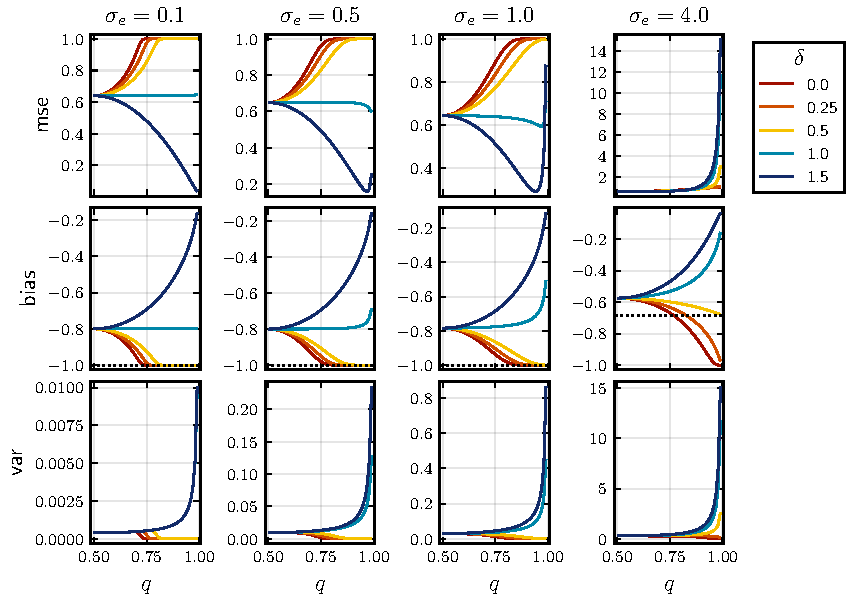
\includegraphics[]{plots/bias-var-onedim.pdf}
  \caption{%
    Bias, variance, and mean-squared error for a one-dimensional lasso problem.
    Note that \(\delta = 0\) corresponds to the case of no scaling, \(\delta = 1/2\) corresponds
    to standardization, and \(\delta = 1\) corresponds to scaling with the variance. The dotted
    lines represent the asymptotic bias of the lasso estimator in the case of \(\delta = 1/2\).
  }
  \label{fig:bias-var-onedim-lasso}
\end{figure}


% We assume now that all the entries in \(\vec{x}\) are generated from a Bernoulli-distributed random variable with parameter \(q\). In this case, the explicit solution to the one-variable elastic net problem is
% \[
%   \E \hat\beta = \frac{\st{\left( n\beta q(1-q) ; \lambda_1\right)}}{\sqrt{q(1-q)} \left(n + (1-\alpha)\lambda\right)}
% \]
% This means that the expected value of the coefficient is sensitive to the class balance in the problem. As \(q\) goes to 0 or 1, the expected value of the coefficient goes to 0 as long as \(\alpha > 0\). When \(\alpha = 0\), on the other hand, the coefficient is unaffected by the class imbalance, and will just, due to the ridge penalty, be a scaled version of the ordinary least squares coefficient.

\subsection{Two-Dimensional Problem}

The previous section served only to introduce some of the main results. Here, we check if they persist when we mix continuous and binary features.

Let us start by assuming that we have a two-dimensional problem and that \(x_{i1} \sim \bernoulli(p)\) and \(x_{i2} \sim \normal(0, 1)\) with no dependence between either the features or the observations. When \(q = 0.5\), the classes are completely balanced, and the population standard deviations become 0.5 and 1 for \(\vec{x}_2\) and \(\vec{x}_1\) respectively. And if we choose to normalize with mean and standard deviation, then, after standardization, values for \(\vec{x}_2\) will lie between 0 and 2, with a standard deviation of 1. For \(\vec{x}_2\), 69\% of the values will lie between an equally spaced range, -1 to 1, and the standard deviation will of course also be 1. If the true model is \(y = \mat{X}\vec{\beta}\) and \(\beta = [1,1]^\T\), then shrinkage will be applied equally across the coefficients of the two features.

\subsubsection{Lasso}
Consider the two dimensional problem

\[
  \frac 1 2 \lVert \vec{y} - \vec{x}_1 \beta_1 -\vec{x}_1 \beta_1 \rVert_2^2 + \lambda \left( | \beta_1 | + |\beta_2| \right).
\]
Assume without loss of generality that $|\mv{y}^\T\mv{x}_1|> |\mv{y}^\T\mv{x}_2|$ (what about equal?)
\begin{proof}
  Note that the problem can be reformulated as
  \[ l(\mv{\beta}) =
    \frac 1 2 \begin{bmatrix}
      \beta_1 \\ \beta_2
    \end{bmatrix}^\T \mv{H} \begin{bmatrix}
      \beta_1 \\ \beta_2
    \end{bmatrix}  -
    \mv{b}^\T \begin{bmatrix}
      \beta_1 \\ \beta_2
    \end{bmatrix} + \lambda  \mv{1}^\T \left| \begin{bmatrix}
      \beta_1 \\ \beta_2
    \end{bmatrix}  \right|.
  \]
  where
  $$
    \mv{b} = \begin{bmatrix}
      \mv{y}^\T \mv{x}_1 & \mv{y}^\T \mv{x}_2
    \end{bmatrix} , \mv{H}  =
    \begin{bmatrix}
      \mv{x}_1^\T \mv{x}_1 & \mv{x}_1^\T \mv{x}_2 \\
      \mv{x}_2^\T \mv{x}_1 & \mv{x}_2^\T \mv{x}_2 \\
    \end{bmatrix} .
  $$
  The first we do is standardize the problem by considering the variable
  $$
    \begin{bmatrix}
      \tilde	\beta_1 \\ \tilde \beta_2
    \end{bmatrix} =  \begin{bmatrix}
      \sqrt{H_{11}} & 0             \\
      0             & \sqrt{H_{22}}
    \end{bmatrix} \begin{bmatrix}
      \beta_1 \\ \beta_2
    \end{bmatrix},
  $$
  Now the transformed problem is
  \[ l( \mv{\tilde \beta }) =
    \frac 1 2 \begin{bmatrix}
      \tilde	\beta_1 \\ \tilde \beta_2
    \end{bmatrix}^\T   \mv{ \tilde H} \begin{bmatrix}
      \tilde	\beta_1 \\  \tilde\beta_2
    \end{bmatrix}
    -  \mv{\tilde b}^\T \begin{bmatrix}
      \tilde	\beta_1 \\ \tilde \beta_2
    \end{bmatrix} + {\tilde \lambda}^\T \left| \begin{bmatrix}
      \tilde	\beta_1 \\ \tilde \beta_2
    \end{bmatrix}  \right|.
  \]
  where now
  $$
    \mv{ \tilde b} = \begin{bmatrix}
      \frac{\mv{y}^\T \mv{x}_1}{\sqrt{\mv{x}_1^\T \mv{x}_1}} \\ \frac{\mv{y}^\T \mv{x}_2}{\sqrt{\mv{x}_2^\T \mv{x}_2}}
    \end{bmatrix} , \mv{ \tilde H}  =
    \begin{bmatrix}
      1    & \rho \\
      \rho & 1    \\
    \end{bmatrix}, \tilde \lambda  = \lambda  \begin{bmatrix}
      \frac{1}{\sqrt{\mv{x}_1^\T \mv{x}_1}} \\ \frac{1}{\sqrt{\mv{x}_2^\T \mv{x}_2}}
    \end{bmatrix} .
  $$
  The sub differential of $ l( \mv{\tilde \beta }) $ is equal to
  $$
    \partial l( \mv{\tilde \beta })  = \mv{ \tilde H} \begin{bmatrix}
      \tilde	\beta_1 \\  \tilde\beta_2
    \end{bmatrix}  -   \mv{\tilde b}  + {\tilde \lambda} \cdot \partial \left| \begin{bmatrix}
      \tilde	\beta_1 \\ \tilde \beta_2
    \end{bmatrix}  \right|.
  $$

  CASE 0: all zero.
  CASE 1:
  First consider the situation where only one $\tilde \beta$ is non-zero. Assume that the first coeffienct is non-zero,then $\hat \beta_1 =  \tilde b_1 -  {\tilde \lambda}_1 sign( \tilde b_1 )$. The gradient of the likelihood of the second component is
  $$
    \rho \hat \beta_1  -  \tilde b_2 \in [-\tilde \lambda_2,\tilde \lambda_2 ]
  $$
\end{proof}

\subsubsection{Class Imbalances}

As long as the classes are balanced, the procedure we used in the previous section, standardization, will yield unbiased estimates of the two coefficients. But what if the classes of the binary feature are imbalanced? That is, what if \(q\) is larger than \(0.5\)? It turns out that the results vary depending on the type of penalty used.

\subsection{Which Predictor Enters First?}

Given our previous results on shrinkage of coefficients of binary features, a natural follow-up question is: how large does the true regression coefficient of a binary feature need to be in order to still be selected?

To begin to probe this question, we first bring the following standard result to attention.

\begin{proposition}
  The first predictor to enter the elastic net path is given by
  \[
    \argmax_j\left| \tilde{\vec{x}}_j^\T\left(\vec{y} - \frac{1}{n}\sum_i y_i \right)\right|.
  \]
\end{proposition}
\begin{proof}
  The proof is a simple consequence of the KKT conditions for the elastic net problem. The first predictor to enter the path is the one that has the largest gradient of the objective function at the origin.
\end{proof}

If we expand the argument inside the absolute value operator, we have
\[
  \tilde{\vec{x}}_j^\T\left( \vec{y} - \frac{1}{n}\ones{}^\T \vec{y}\right) = \frac{1}{s_j}\left(\vec{x}_j^\T \vec{y} - \frac{1}{n}\ones^\T \vec{y} \ones^\T \vec{x}_j\right)
\]
Assuming that \(\vec{y} = \mat{X}\vec{\beta}^* + \vec{\varepsilon}\) as before, and that the entries of each feature \(\vec{x}_j\) in the design matrix are sampled independently and identically from a corresponding random variable \(X_j\), we can take the expected value of the expression, yielding \textcolor{red}{this is only true if $X_j$ is independent of $s_j$ and also $\E \frac{1}{s_j} \neq \frac{1}{\E s_j}$}
% FIXME: We're not really allowed to compute the exected value like this. So we need to motivate it somehow. Maybe assume that the scaling and centering factors are fixed or something?
\[
  \frac{1}{\E s_j}\left( n \beta^*_j \E X_j^2 - n \beta^*_j (\E X_j)^2 \right) = \frac{n \beta^*_j\var X_j}{\E s_j}.
\]
Assuming that we have two features in our design, they enter the model at exactly the same time if
\[
  \begin{aligned}
    \frac{n \beta^*_1\var X_1}{\E s_1} & = \frac{n \beta^*_2\var X_2}{\E s_2} \implies                     \\
    \beta^*_1                          & = \frac{\beta^*_2\var X_2}{\E s_2} \times \frac{\E s_1}{\var X_1}
  \end{aligned}
\]

Next, assume that \(X_1 \sim \bernoulli{(q)}\) and \(X_2 \sim \normal{(0, 0.5)}\) and that \(\beta^*_2 = 1\). In this case, how large does \(\beta^*_1\) be in order for the first feature to enter the model at the same time as the second one?

First, observe that \(\var{X_1} = q(1 - q)\) and \(\var{X_2} = 0.25\). In other words, we have
\begin{equation}
  \label{eq:beta1star}
  \beta^*_1 = \frac{\E s_1}{4q(1-q)\E s_2}
\end{equation}

\paragraph{Standardization} If the features are standardized, then \Cref{eq:beta1star} is
\[
  \beta^*_1 = \frac{1}{2\sqrt{q(1-q)}}
\]

If the classes are balanced, \(q = 0.5\), then this means that the coefficients are expected to be the same. If, however, for instance \(q = 0.1\), then the coefficient for the binary feature needs to be 5/3 times larger than the continuous one to enter the model at the same time. If \(q=0.01\), the respective figure is roughly five. \textcolor{red}{Is there a difference if one would have a $X_1 \sim \mathcal{N}\left(0,q(1-q) \right)?$ }

\paragraph{Max-Abs Normalization} In this case, we get
\[
  \beta^*_1 = \frac{1}{q(1 - q)} \times \frac{1}{\E \max | X_{12}, \dots,  X_{n2} |}.
\]

\paragraph{Min-Max Normalization} In this case, we get
\[
  \beta^*_1 = \frac{1}{q(1 - q)} \times \frac{1}{\E \left(\max | X_{12}, \dots,  X_{n2}| - \min | X_{12}, \dots,  X_{n2} |\right)}.
\]

\subsection{Relative Size of Predictors in Model}

The next question we now ask ourselves is: given that both features are in the model, what are their respective sizes given differences in class balance (\(q\))?

To begin to answer this question, we conduct simulations on a two-dimensional problem. Along with our previous reasoning, we sample one feature from \(\normal(0, 0.5)\) and the other from \(\bernoulli(q)\), varying \(q\) in \([0.5, 0.99]\) to simulate the effect of class imbalance on the estimates from the model. We compare four different strategies of normalization:
\begin{description}
  \item[Mean-Std] Standardization
  \item[Mean-StdVar] Mean centering and scaling the normal feature by standard deviation and the binary feature by variance
  \item[Mean-Var] Mean centering and scaling each feature by its variance
  \item[None] No normalization
\end{description}

The results~(\Cref{fig:lasso-ridge-comparison}) show that when it comes to ridge, standardization creates class balance-insensitive estimates, whereas for the lasso, this is not the case. For the lasso, it is instead the Mean-StdVar and Mean-Var normalization methods that generate estimates that are insensitive to class imbalances.

\begin{figure}[htpb]
  \centering
  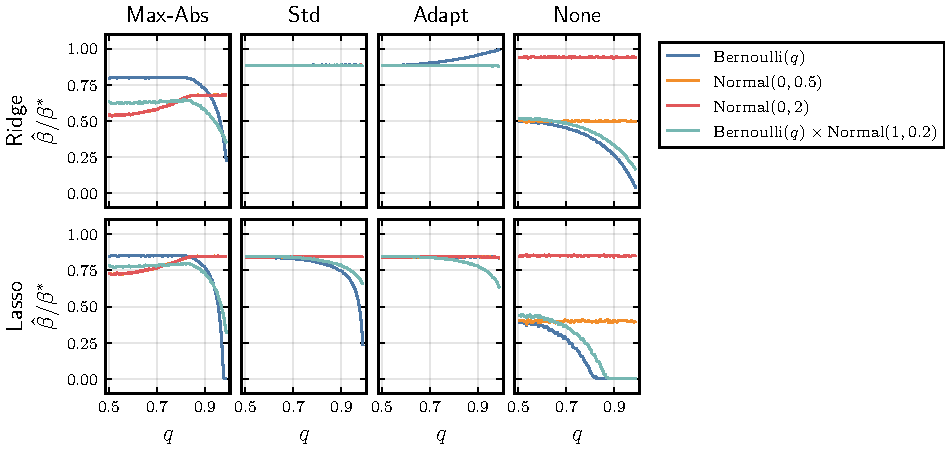
\includegraphics{plots/lassoridge_twodim.pdf}
  \caption{%
    Comparison between lasso and ridge estimators for a two-dimensional problem where one feature is generated from \(\bernoulli(q)\) and the other from \(\normal(0, 0.5)\) and the features are normalized in various ways.}
  \label{fig:lasso-ridge-comparison}
\end{figure}

\subsection{Varying Class Imbalances}

Here, we conduct an experiment on a \(300 \times 500\) design matrix, where the first 20 features are binary and the remaining ones are normally distributed with standard deviation 0.5. We consider four different cases for the class balances:
\begin{description}
  \item[Balanced] All of the signals have a class balance of 0.5.
  \item[Unbalanced] All of the signals have a class balance of 0.9.
  \item[Very Unbalanced] All of the signals have a class balance of 0.99.
  \item[Decreasing] The class balance of the signals decreases geometrically from 0.5 to 0.99.
\end{description}

To conduct the experiment, we generate random data and split it in a 50/50 training/test set split. Then, we select \(lambda\) using 10-fold cross validation on the training set and finally compute mean-squared error on the test set. We repeat this procedure 50 times for each combination of normalization type and class balance behavior.

The results~(\Cref{fig:binary-sim}) show that standardization performs best among the different types of normalization strategies.
% TODO: Expand on this.

\begin{figure}[htpb]
  \centering
  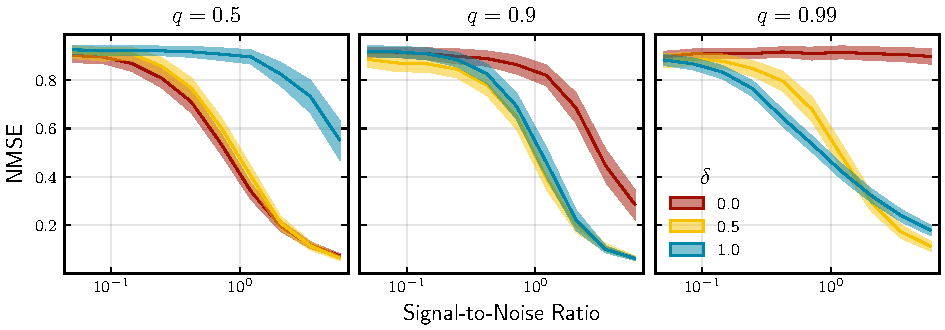
\includegraphics[]{plots/binary_data_sim.pdf}
  \caption{%
    Mean-squared error of \(y - \hat y\) for different types of normalizaion and types of class imbalances in a data set with only binary features.
  }
  \label{fig:binary-sim}
\end{figure}

\begin{figure}[htpb]
  \centering
  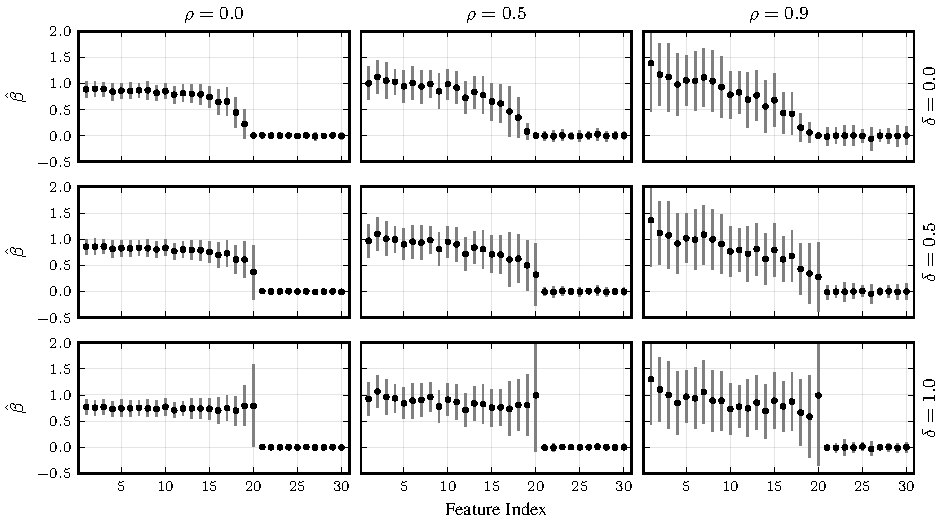
\includegraphics[]{plots/binary_decreasing.pdf}
  \caption{%
    Estimates of the regression coefficients, \(\hat{\vec{\beta}}\), for the first 40 coefficients in the experiment. All of the features are binary and the first 20 features correspond to true signals, with a geometrically decreasing class balance from 0.5 to 0.99. The remaining features have a class balance that's randomly sampled from a uniform distribution with parameters 0.5 and 0.99.}
  \label{fig:binary-decreasing}
\end{figure}

\begin{figure}[htpb]
  \centering
  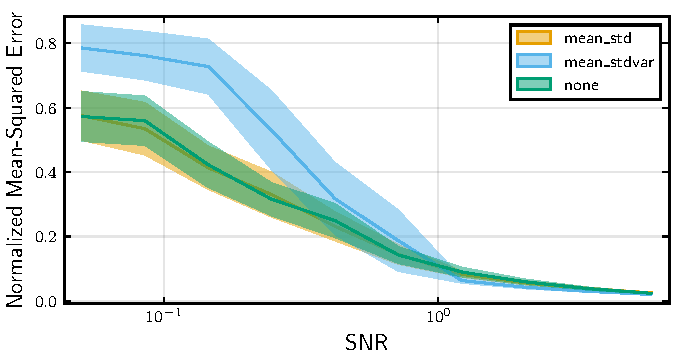
\includegraphics[]{plots/binary_decreasing_snr.pdf}
  \caption{%
    Prediction performance of an experiment with geometrically decreasing class balances for signals and varying signal to noise ratios.
  }
  \label{fig:binary-decreasing-snr}
\end{figure}

\subsection{Mixed Data}

\begin{figure}[htpb]
  \centering
  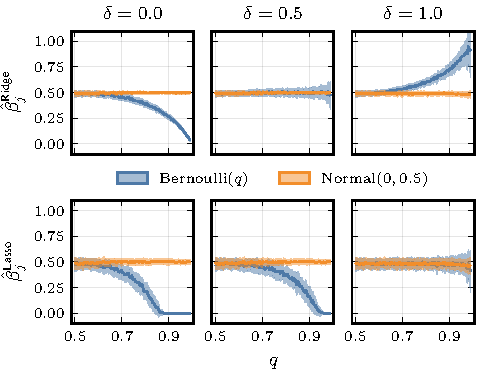
\includegraphics[]{plots/mixed_data.pdf}
  \caption{%
    An experiment with mixed (normal and Bernouli-distributed) data.
  }
  \label{fig:mixed-data}
\end{figure}


\printbibliography

\end{document}
